
\pdfminorversion=4 % for acroread
%\documentclass[aspectratio=169,t,xcolor={usenames,dvipsnames}]{beamer}
\documentclass[aspectratio=169,t,handout,xcolor={usenames,dvipsnames}]{beamer}
\usepackage{../beamerstyle}
\usepackage{dsfont}
\usepackage{bm}
\usepackage[english]{babel}
\usepackage[utf8]{inputenc}
\usepackage{graphicx}
\usepackage{algorithm}
\usepackage[ruled,vlined,algo2e,linesnumbered]{algorithm2e}
%\usepackage[boxed,vlined]{algorithm2e}
\usepackage{hyperref}
\usepackage{booktabs}
\usepackage{mathtools}

\usepackage{amsmath,amssymb}
\usepackage{listings}
\lstset{frame=lines,framesep=3pt,numbers=left,numberblanklines=false,basicstyle=\ttfamily\small}

\usepackage{subfig}
\usepackage{multicol}
%\usepackage{appendixnumberbeamer}
%
\usepackage{tcolorbox}

\usepackage{pgfplots}
\usepackage{tikz}
\usetikzlibrary{trees} 
\usetikzlibrary{shapes.geometric}
\usetikzlibrary{positioning,shapes,shadows,arrows,calc,mindmap}
\usetikzlibrary{positioning,fadings,through}
\usetikzlibrary{decorations.pathreplacing}
\usetikzlibrary{intersections}
\usetikzlibrary{positioning,fit,calc,shadows,backgrounds}
\pgfdeclarelayer{background}
\pgfdeclarelayer{foreground}
\pgfsetlayers{background,main,foreground}
\tikzstyle{activity}=[rectangle, draw=black, rounded corners, text centered, text width=8em]
\tikzstyle{data}=[rectangle, draw=black, text centered, text width=8em]
\tikzstyle{myarrow}=[->, thick, draw=black]

% Define the layers to draw the diagram
\pgfdeclarelayer{background}
\pgfdeclarelayer{foreground}
\pgfsetlayers{background,main,foreground}

%\usepackage{listings}
%\lstset{numbers=left,
%  showstringspaces=false,
%  frame={tb},
%  captionpos=b,
%  lineskip=0pt,
%  basicstyle=\ttfamily,
%%  extendedchars=true,
%  stepnumber=1,
%  numberstyle=\small,
%  xleftmargin=1em,
%  breaklines
%}

 
\definecolor{blue}{RGB}{0, 74, 153}

\usetheme{Boadilla}
%\useinnertheme{rectangles}
\usecolortheme{whale}
\setbeamercolor{alerted text}{fg=blue}
\useoutertheme{infolines}
\setbeamertemplate{navigation symbols}{\vspace{-5pt}} % to lower the logo
\setbeamercolor{date in head/foot}{bg=white} % blue
\setbeamercolor{date in head/foot}{fg=white}
\setbeamercolor{author  in head/foot}{bg=white} %blue
\setbeamercolor{title in head/foot}{bg=white} % blue
\setbeamercolor{title}{fg=white, bg=blue}
\setbeamercolor{block title}{fg=white,bg=blue}
\setbeamercolor{block body}{bg=blue!10}
\setbeamercolor{frametitle}{fg=white, bg=blue}
\setbeamercovered{invisible}

\makeatletter
\setbeamertemplate{footline}
{
  \leavevmode%
  \hbox{%
  \begin{beamercolorbox}[wd=.333333\paperwidth,ht=2.25ex,dp=1ex,center]{author in head/foot}%
%    \usebeamerfont{author in head/foot}\insertshortauthor
  \end{beamercolorbox}%
  \begin{beamercolorbox}[wd=.333333\paperwidth,ht=2.25ex,dp=1ex,center]{title in head/foot}%
    \usebeamerfont{title in head/foot}\insertshorttitle
  \end{beamercolorbox}%
  \begin{beamercolorbox}[wd=.333333\paperwidth,ht=2.25ex,dp=1ex,right]{date in head/foot}%
    \usebeamerfont{date in head/foot}\insertshortdate{}\hspace*{2em}
%    \insertframenumber\hspace*{2ex} 
  \end{beamercolorbox}}%
  \vskip0pt%
}
\makeatother

%\pgfdeclareimage[height=1.2cm]{automl}{images/logos/automl.png}
%\pgfdeclareimage[height=1.2cm]{freiburg}{images/logos/freiburg}

%\logo{\pgfuseimage{freiburg}}

\renewcommand{\comment}[1]{
	\noindent
	%\vspace{0.25cm}
	{\color{red}{\textbf{TODO:} #1}}
	%\vspace{0.25cm}
}
\newcommand{\notefh}[1]{\textcolor{red}{\textbf{FH:} #1}}
\renewcommand{\comment}[1]{}
\newcommand{\hide}[1]{}
\newcommand{\cemph}[2]{\emph{\textcolor{#1}{#2}}}

\newcommand{\lit}[1]{{\footnotesize\color{black!60}[#1]}}

\newcommand{\litw}[1]{{\footnotesize\color{blue!20}[#1]}}


\newcommand{\myframe}[2]{\begin{frame}[c]{#1}#2\end{frame}}
\newcommand{\myframetop}[2]{\begin{frame}{#1}#2\end{frame}}
\newcommand{\myit}[1]{\begin{itemize}#1\end{itemize}}
\newcommand{\myblock}[2]{\begin{block}{#1}#2\end{block}}


\newcommand{\votepurple}[1]{\textcolor{Purple}{$\bigstar$}}
\newcommand{\voteyellow}[1]{\textcolor{Goldenrod}{$\bigstar$}}
\newcommand{\voteblue}[1]{\textcolor{RoyalBlue}{$\bigstar$}}
\newcommand{\votepink}[1]{\textcolor{Pink}{$\bigstar$}}

\newcommand{\diff}{\mathop{}\!\mathrm{d}}
\newcommand{\refstyle}[1]{{\small{\textcolor{gray}{#1}}}}
\newcommand{\hands}[0]{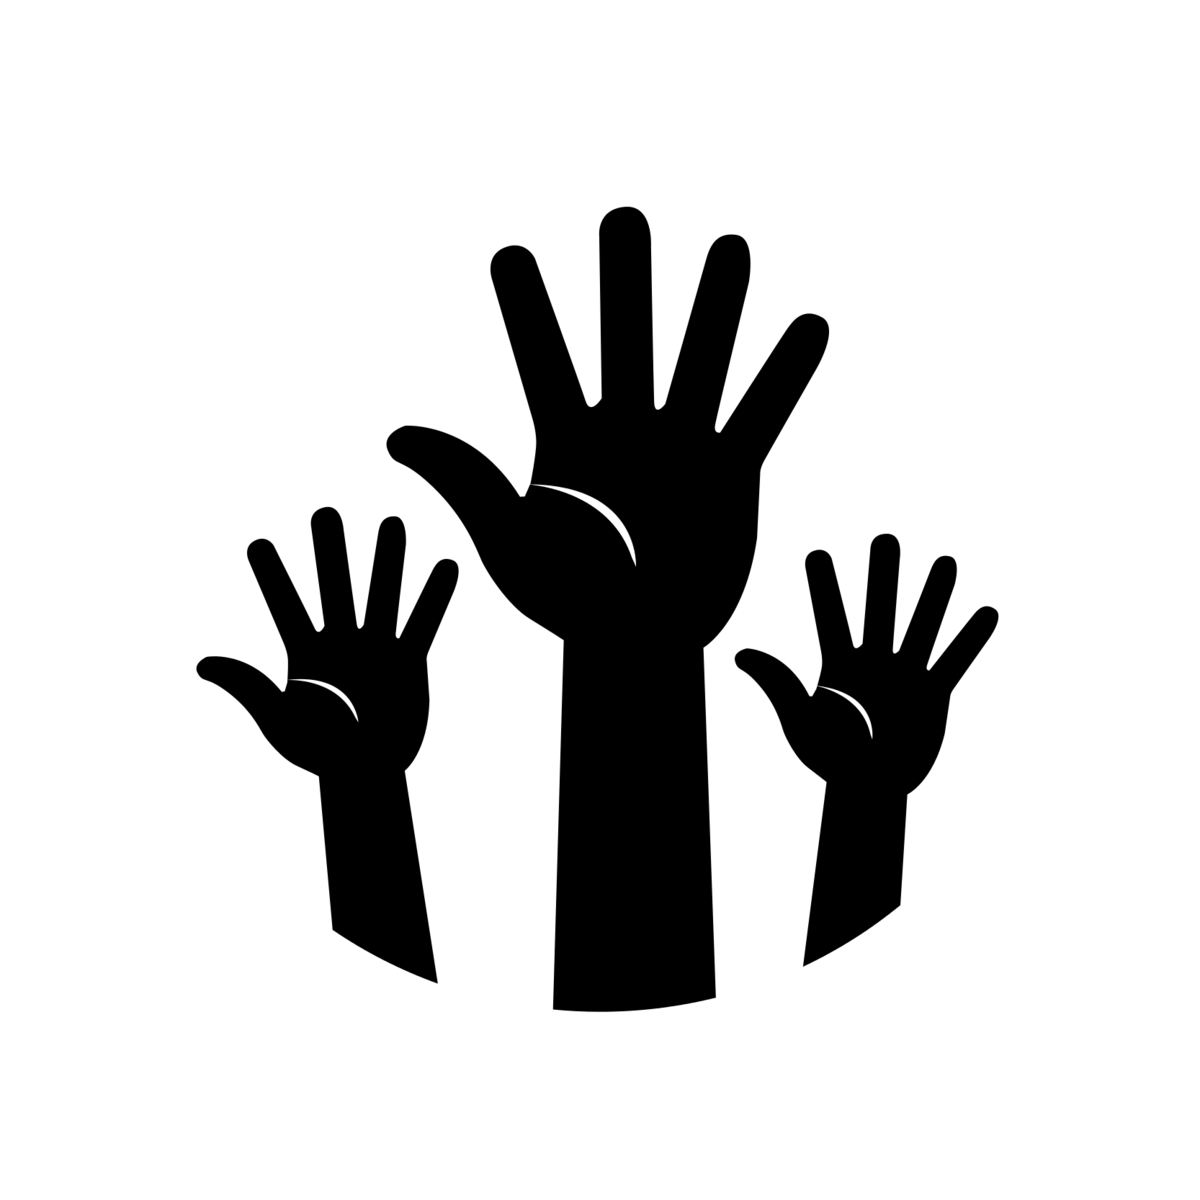
\includegraphics[height=1.5em]{images/hands}}
\newcommand{\transpose}[0]{{\textrm{\tiny{\sf{T}}}}}
\newcommand{\norm}{{\mathcal{N}}}
\newcommand{\cutoff}[0]{\kappa}
\newcommand{\instD}[0]{\dataset}
\newcommand{\insts}[0]{\mathcal{I}}
\newcommand{\inst}[0]{i}
\newcommand{\instI}[1]{i^{(#1)}}

% Iteration specific instance of variable/function/anything
% Introduced in the BO section, but moved up here to make it available within other macros
\newcommand{\iter}[2][\bocount]{{#2}^{(#1)}}

%--------HPO parameter macros-----------

% Parameter Configuration Space
\newcommand{\pcs}[0]{\pmb{\Lambda}}

% ???
\newcommand{\bx}[0]{\conf}

% Parameter Configuration
\newcommand{\conf}[0]{\pmb{\lambda}}

% Final Configuration
\newcommand{\finconf}[0]{\pmb{\hat{\lambda}}}

% Configuration corresponding to a given iteration -- better use \iter!
\newcommand{\confI}[1]{{\conf}^{(#1)}}

% Default Configuration
\newcommand{\defconf}[0]{{\conf}_{\text{def}}}

% Incumbent Configuration
\newcommand{\incumbent}[1][\bocount]{\iter[#1]{\finconf}}

% Optimal Configuration
\newcommand{\optconf}[0]{{\conf}^*}

% Configuration Space
\newcommand{\confs}[0]{\pcs}

%----------------------------------------

%\newcommand{\vlambda}[0]{\bm{\lambda}}
%\newcommand{\vLambda}[0]{\bm{\Lambda}}
\newcommand{\dataset}[0]{\mathcal{D}}
\newcommand{\datasets}[0]{\mathbf{D}}
\newcommand{\loss}[0]{L}
\newcommand{\risk}{\mathcal{R}}
\newcommand{\riske}{\mathcal{R}_{\text{emp}}}
\newcommand{\cost}[0]{c}
\newcommand{\costI}[1]{c^{(#1)}}

% Gaussian Process
\newcommand{\gp}{\mathcal{G}}
% Family of Objective Functions
\newcommand{\objF}{F}

%---------------BO Macros------------------

% BO loop counter
\newcommand{\bocount}{t}
% BO loop counter max, the counter runs from 1 to this value
\newcommand{\bobudget}{T}
% BO loop observation
\newcommand{\obs}[1][\conf]{\cost({#1})}
% BO loop observation space
\newcommand{\obsspace}{\mathcal{Y}}
% BO loop next observation
\newcommand{\bonextobs}{\obs[\iter{\conf}]}
% Acquisition Function, no args
\newcommand{\acq}{u}
% Standard Normal PDF
\newcommand{\pdf}{\phi}
% Standard Normal CDF
\newcommand{\cdf}{\Phi}
% Mean
\newcommand{\mean}{\mu}
% Standard Deviation
\newcommand{\stddev}{\sigma}
% Variance
\newcommand{\variance}{\sigma^2}
% Noise
\newcommand{\noise}{\nu}
% BO loop next selected sample
\newcommand{\bonextsample}{\confI{\bocount}}

% Single hyperparameter
\newcommand{\hyperparam}{\lambda}

% Single hyperparameter within a hyperparameter configuration
\newcommand{\hyperparami}[1][i]{{\hyperparam}_#1}

% Full definition of final configuration
\newcommand{\finconffull}{\incumbent[\bobudget]}

% Dataset
\newcommand{\datasetHPO}{{\dataset}_{HPO}}

% Dataset definition
\newcommand{\datasetHPOdef}{{\langle \bonextsample,\,\bonextobs \rangle}_{\bocount=1}^{\bobudget}}

% Double Display Fraction, forces large displays for everything in numerator and denominator
\newcommand\ddfrac[2]{\frac{\displaystyle #1}{\displaystyle #2}}

% Conditional Probability "Given That" Relation, source:https://tex.stackexchange.com/a/141685/205886
\newcommand\given[1][]{\:#1\vert\:}

% Expectation as a math operator
\DeclareMathOperator*{\E}{\mathbb{E}}

% Citation 
\newcommand{\source}[1]{
    \begin{flushright}
    	Source: \lit{#1}
    \end{flushright}
}
%-------------------------------------------

%Real numbers set
\newcommand{\realnum}{\mathbb{R}}
%Configuration space - do not use
%\newcommand{\configspace}{\Theta}
%Instances - do not use
%\newcommand{\instances}{\mathcal{I}}
%Expected value
\newcommand{\expectation}{\mathbb{E}}
%Kernel
\newcommand{\kernel}{\kappa}
%Constraint function
\newcommand{\constraintf}{c}
%Normal distribution
\newcommand{\normaldist}{\mathcal{N}}

% \renewcommand{\vec}[1]{\mathbf{#1}}
\newcommand{\hist}[0]{\dataset_{\text{Hist}}}
\newcommand{\param}[0]{p}
\newcommand{\algo}[0]{\mathcal{A}}
\newcommand{\algos}[0]{\mathbf{A}}
%\newcommand{\nn}[0]{N}
\newcommand{\feats}[0]{\mathcal{X}_{\text{meta}}}
\newcommand{\feat}[0]{\x_{\text{meta}}}
%\newcommand{\cluster}[0]{\vec{h}}
%\newcommand{\clusters}[0]{\vec{H}}
\newcommand{\perf}[0]{\mathbb{R}}
%\newcommand{\surro}[0]{\mathcal{S}}
\newcommand{\surro}[0]{\hat{\cost}}
\newcommand{\func}[0]{f}
\newcommand{\epm}[0]{\surro}
\newcommand{\portfolio}[0]{\mathbf{P}}
\newcommand{\schedule}[0]{\mathcal{S}}

% Machine Learning
\newcommand{\mdata}[0]{\dataset_{\text{meta}}}
\newcommand{\datasettrain}[0]{\dataset_{\text{train}}}
\newcommand{\datasetval}[0]{\dataset_{\text{val}}}
\newcommand{\datasettest}[0]{\dataset_{\text{test}}}
\newcommand{\x}[0]{\mathbf{x}}
\newcommand{\y}[0]{y}
\newcommand{\xI}[1]{\mathbf{x}^{(#1)}}
\newcommand{\yI}[1]{y^{(#1)}}
\newcommand{\fx}{f(\mathbf{x})}  % f(x), continuous prediction function
\newcommand{\Hspace}{\mathcal{H}} % hypothesis space where f is from
\newcommand{\fh}{\hat{f}}       % f hat, estimated prediction function

% Deep Learning
\newcommand{\weights}[0]{\theta}
\newcommand{\metaweights}[0]{\phi}


% reinforcement learning
\newcommand{\policies}[0]{\mathbf{\Pi}}
\newcommand{\policy}[0]{\pi}
\newcommand{\actionRL}[0]{a}
\newcommand{\stateRL}[0]{s}
\newcommand{\statesRL}[0]{\mathcal{S}}
\newcommand{\rewardRL}[0]{r}
\newcommand{\rewardfuncRL}[0]{\mathcal{R}}

\RestyleAlgo{algoruled}
\DontPrintSemicolon
\LinesNumbered
\SetAlgoVlined
\SetFuncSty{textsc}

\SetKwInOut{Input}{Input}
\SetKwInOut{Output}{Output}
\SetKw{Return}{return}

%\newcommand{\changed}[1]{{\color{red}#1}}

%\newcommand{\citeN}[1]{\citeauthor{#1}~(\citeyear{#1})}

\renewcommand{\vec}[1]{\mathbf{#1}}
\DeclareMathOperator*{\argmin}{arg\,min}
\DeclareMathOperator*{\argmax}{arg\,max}

%\newcommand{\aqme}{\textit{AQME}}
%\newcommand{\aslib}{\textit{ASlib}}
%\newcommand{\llama}{\textit{LLAMA}}
%\newcommand{\satzilla}{\textit{SATzilla}}
%\newcommand{\satzillaY}[1]{\textit{SATzilla'{#1}}}
%\newcommand{\snnap}{\textit{SNNAP}}
%\newcommand{\claspfolioTwo}{\textit{claspfolio~2}}
%\newcommand{\flexfolio}{\textit{FlexFolio}}
%\newcommand{\claspfolioOne}{\textit{claspfolio~1}}
%\newcommand{\isac}{\textit{ISAC}}
%\newcommand{\eisac}{\textit{EISAC}}
%\newcommand{\sss}{\textit{3S}}
%\newcommand{\sunny}{\textit{Sunny}}
%\newcommand{\ssspar}{\textit{3Spar}}
%\newcommand{\cshc}{\textit{CSHC}}
%\newcommand{\cshcpar}{\textit{CSHCpar}}
%\newcommand{\measp}{\textit{ME-ASP}}
%\newcommand{\aspeed}{\textit{aspeed}}
%\newcommand{\autofolio}{\textit{AutoFolio}}
%\newcommand{\cedalion}{\textit{Cedalion}}
\newcommand{\fanova}{\textit{fANOVA}}
\newcommand{\sbs}{\textit{SB}}
\newcommand{\oracle}{\textit{VBS}}

% like approaches
\newcommand{\claspfoliolike}[1]{\texttt{claspfolio-#1-like}}
\newcommand{\satzillalike}[1]{\texttt{SATzilla'#1-like}}
\newcommand{\isaclike}{\texttt{ISAC-like}}
\newcommand{\ssslike}{\texttt{3S-like}}
\newcommand{\measplike}{\texttt{ME-ASP-like}}

\newcommand{\irace}{\textit{I/F-race}}
\newcommand{\gga}{\textit{GGA}}
\newcommand{\smac}{\textit{SMAC}}
\newcommand{\paramils}{\textit{ParamILS}}
\newcommand{\spearmint}{\textit{Spearmint}}
\newcommand{\tpe}{\textit{TPE}}


\usepackage{pifont}
\newcommand{\itarrow}{\mbox{\Pisymbol{pzd}{229}}}
\newcommand{\ithook}{\mbox{\Pisymbol{pzd}{52}}}
\newcommand{\itcross}{\mbox{\Pisymbol{pzd}{56}}}
\newcommand{\ithand}{\mbox{\raisebox{-1pt}{\Pisymbol{pzd}{43}}}}

%\DeclareMathOperator*{\argmax}{arg\,max}

\newcommand{\ie}{{\it{}i.e.\/}}
\newcommand{\eg}{{\it{}e.g.\/}}
\newcommand{\cf}{{\it{}cf.\/}}
\newcommand{\wrt}{\mbox{w.r.t.}}
\newcommand{\vs}{{\it{}vs\/}}
\newcommand{\vsp}{{\it{}vs\/}}
\newcommand{\etc}{{\copyedit{etc.}}}
\newcommand{\etal}{{\it{}et al.\/}}

\newcommand{\pscProc}{{\bf procedure}}
\newcommand{\pscBegin}{{\bf begin}}
\newcommand{\pscEnd}{{\bf end}}
\newcommand{\pscEndIf}{{\bf endif}}
\newcommand{\pscFor}{{\bf for}}
\newcommand{\pscEach}{{\bf each}}
\newcommand{\pscThen}{{\bf then}}
\newcommand{\pscElse}{{\bf else}}
\newcommand{\pscWhile}{{\bf while}}
\newcommand{\pscIf}{{\bf if}}
\newcommand{\pscRepeat}{{\bf repeat}}
\newcommand{\pscUntil}{{\bf until}}
\newcommand{\pscWithProb}{{\bf with probability}}
\newcommand{\pscOtherwise}{{\bf otherwise}}
\newcommand{\pscDo}{{\bf do}}
\newcommand{\pscTo}{{\bf to}}
\newcommand{\pscOr}{{\bf or}}
\newcommand{\pscAnd}{{\bf and}}
\newcommand{\pscNot}{{\bf not}}
\newcommand{\pscFalse}{{\bf false}}
\newcommand{\pscEachElOf}{{\bf each element of}}
\newcommand{\pscReturn}{{\bf return}}

%\newcommand{\param}[1]{{\sl{}#1}}
\newcommand{\var}[1]{{\it{}#1}}
\newcommand{\cond}[1]{{\sf{}#1}}
%\newcommand{\state}[1]{{\sf{}#1}}
%\newcommand{\func}[1]{{\sl{}#1}}
\newcommand{\set}[1]{{\Bbb #1}}
%\newcommand{\inst}[1]{{\tt{}#1}}
\newcommand{\myurl}[1]{{\small\sf #1}}

\newcommand{\Nats}{{\Bbb N}}
\newcommand{\Reals}{{\Bbb R}}
\newcommand{\extset}[2]{\{#1 \; | \; #2\}}

\newcommand{\vbar}{$\,\;|$\hspace*{-1em}\raisebox{-0.3mm}{$\,\;\;|$}}
\newcommand{\vendbar}{\raisebox{+0.4mm}{$\,\;|$}}
\newcommand{\vend}{$\,\:\lfloor$}


\newcommand{\goleft}[2][.7]{\parbox[t]{#1\linewidth}{\strut\raggedright #2\strut}}
\newcommand{\rightimage}[2][.3]{\mbox{}\hfill\raisebox{1em-\height}[0pt][0pt]{\includegraphics[width=#1\linewidth]{#2}}\vspace*{-\baselineskip}}





\newcommand{\q}[0]{\mathbf{q}}

%The following might look confusing but allows us to switch the notation of the optimization problem independently from the notation of the hyper parameter optimization
\newcommand{\xx}{\conf} %x of the optimizer
\newcommand{\xxi}[1][i]{\lambda_{#1}} %i-th component of xx (not confuse with i-th individual)
\newcommand{\XX}{\pcs} %search space / domain of f
\newcommand{\f}{\cost} %objective function
%\newcommand{\y}{\cost} %outcome of objective function

\title[AutoML: Overview]{Multi-criteria Optimization}
\subtitle{Evolutionary Approaches}
%TODO: change authors!
\author[Bernd Bischl]{\underline{Bernd Bischl} \and Frank Hutter \and Lars Kotthoff\newline \and Marius Lindauer \and Joaquin Vanschoren}
\institute{}
\date{}



% \AtBeginSection[] % Do nothing for \section*
% {
%   \begin{frame}{Outline}
%     \bigskip
%     \vfill
%     \tableofcontents[currentsection]
%   \end{frame}
% }

\begin{document}

	\maketitle




\begin{frame}[allowframebreaks]{A-posteriori methods and evolutionary algorithms}

Evolutionary multi-objective algorithms (EMOAs) evolve a diverse population over time to approximate the Pareto front. 

\begin{columns}
\begin{column}{0.3\textwidth}
\begin{center}
\begin{figure}
\centering
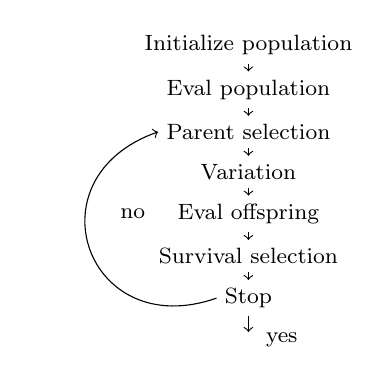
\begin{tikzpicture}[node distance=-1.8cm, auto,]
%nodes
\begin{footnotesize}
\node (init) {Initialize population};
\node[below = 0.1cm of init](rating1) {Eval population};
\node[below = 0.1cm of rating1](selection1) {Parent selection};
\node[below = 0.1cm of selection1](variation) {Variation};
\node[below = 0.1cm of variation](rating2) {Eval offspring};
\node[below = 0.1cm of rating2](selection2) {Survival selection};
\node[below = 0.1cm of selection2](stop) {Stop};
\node[below = 0.2cm of stop](dummy2) {};
\node[below = 0.2cm of stop](dummy3) {};
\node[right = 0.01cm of dummy3](dummy4) {yes};
\node[left = 0.2cm of rating2](dummy1) {no};
\draw[->] (init) to (rating1) node[midway, above]{};
\draw[->] (rating1) to (selection1) node[midway, above]{};
\draw[->] (selection1) to (variation) node[midway, above]{};
\draw[->] (variation) to (rating2) node[midway, above]{};
\draw[->] (rating2) to (selection2) node[midway, above]{};
\draw[->] (selection2) to (stop) node[midway, above]{};
\draw[->] (stop) to (dummy2) node[midway, above]{};
\draw[->] (stop) to [bend left=90, looseness=2](selection1) node[midway, above]{};
\end{footnotesize}
\end{tikzpicture}
\end{figure}
\end{center}
\begin{footnotesize}
\end{footnotesize}
\end{column}
    
\begin{column}{0.7\textwidth}
\begin{center}
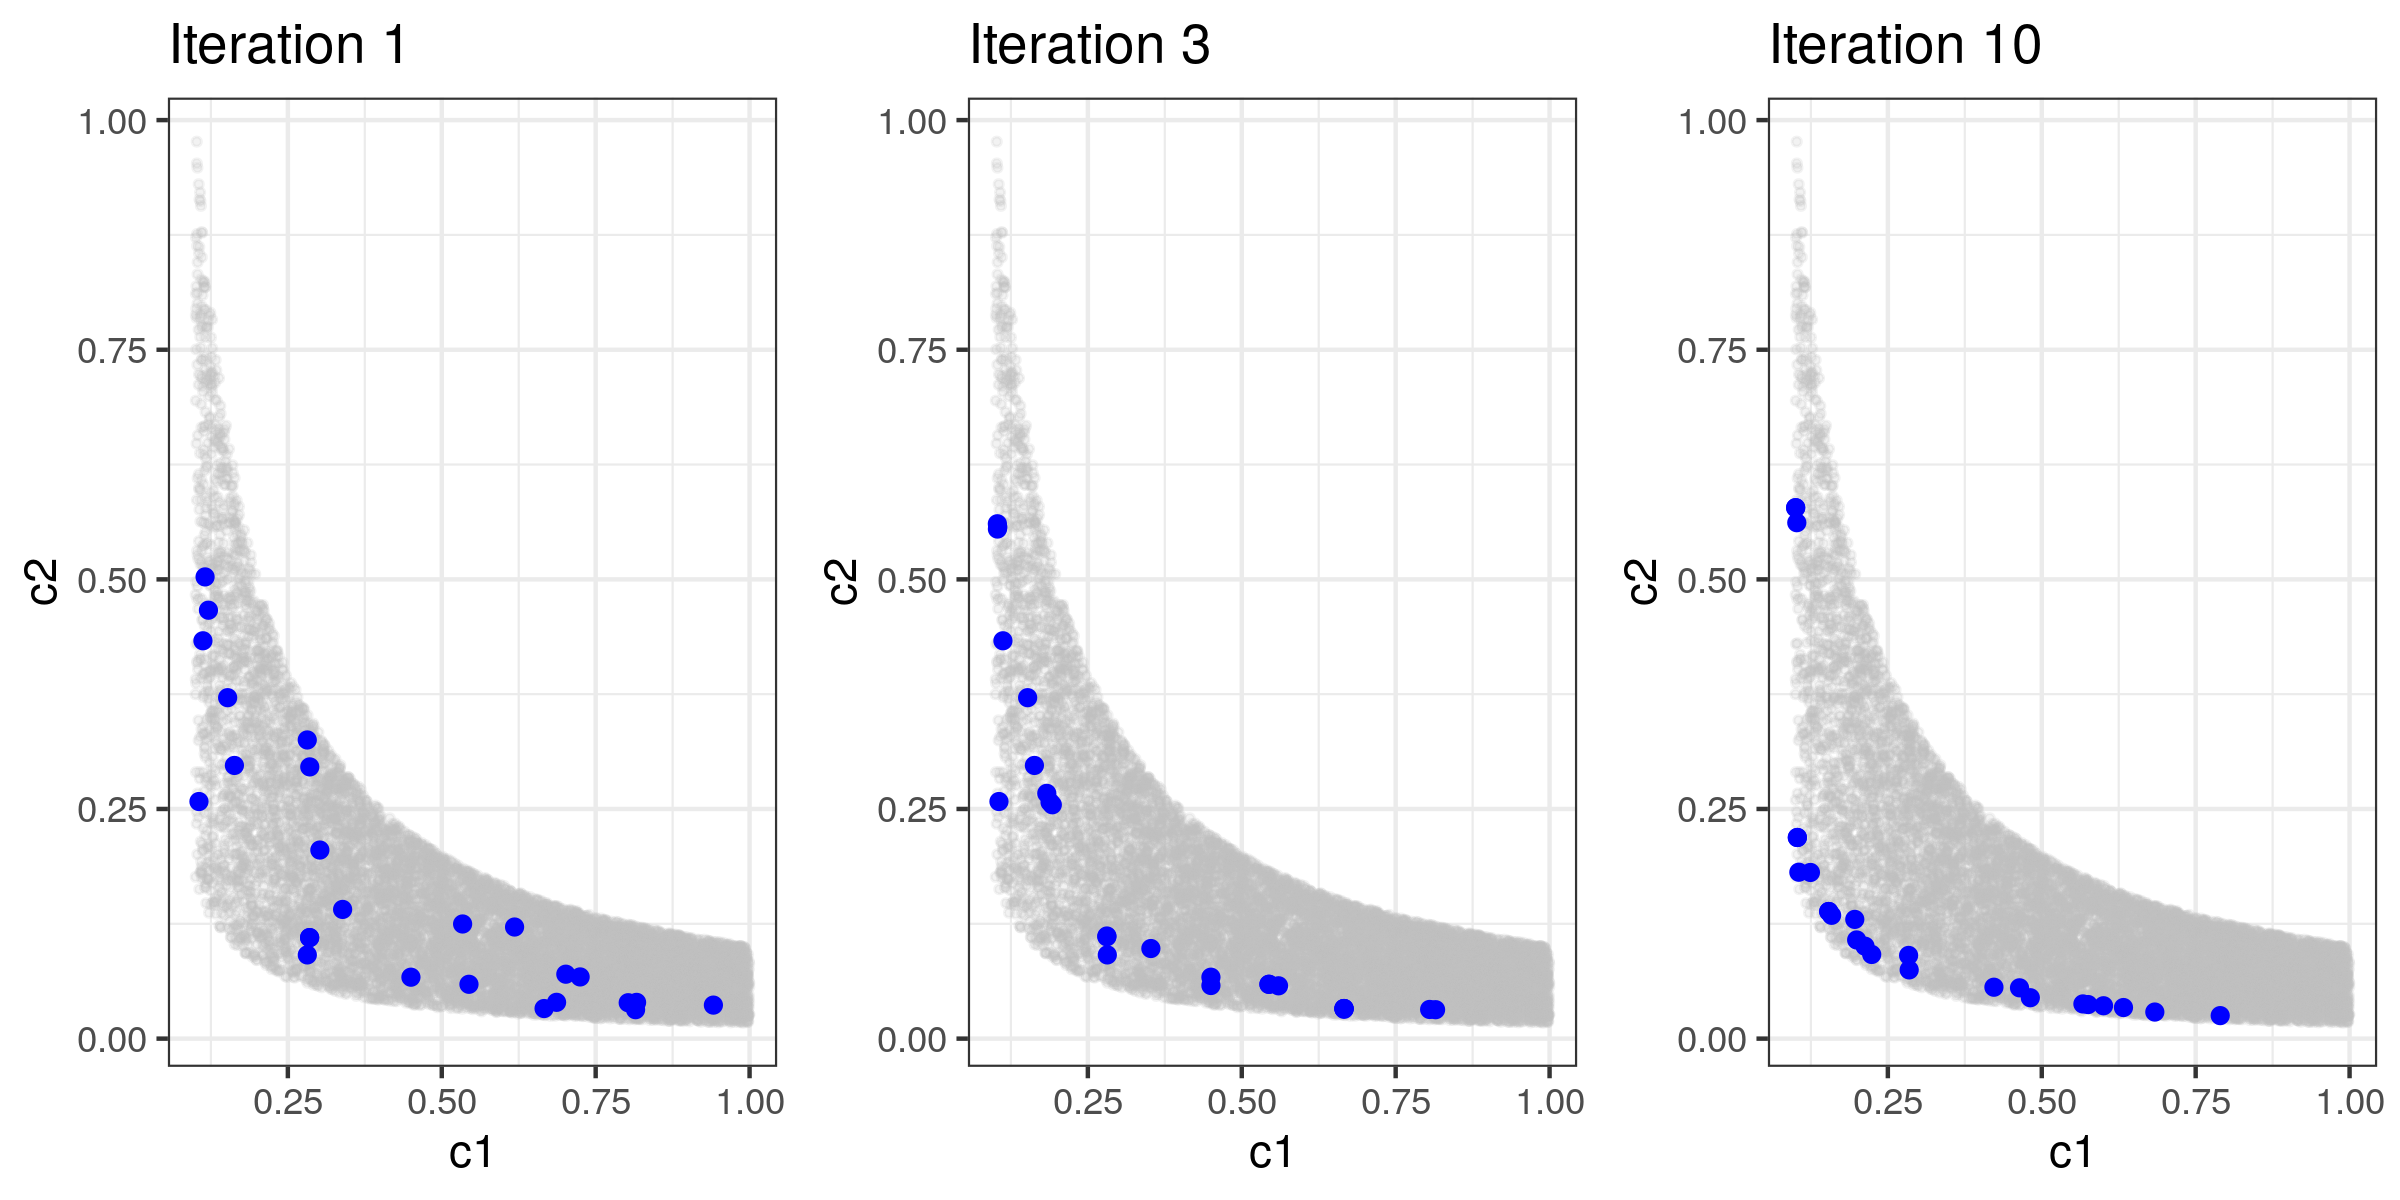
\includegraphics[width = 0.9\textwidth]{images/NSGA2_steps.png}
\end{center}
\end{column}
\end{columns}
% Image of the function (grey) and target function values $(\cost_1(\), \cost_2(\x))$ for $\x \in \mathcal{P}_i, i = 1, 3, 10$ (blue).

\framebreak

\begin{algorithm}[H]
  \begin{center}
  \caption{Basic EA template loop}
      \begin{algorithmic}[1]
          \STATE Init and eval population $\mathcal{P}_0 \subset \XX$ with $|\mathcal{P}| = \mu$ 
      \STATE $t \leftarrow 0$
      \REPEAT
        \STATE Select parents and generate offspring $\mathcal{Q}_t$ with $|\mathcal{Q}_t| = \lambda$
        \STATE Select $\mu$ survivors $\mathcal{P}_{t + 1}$ 
 		\STATE $t \leftarrow t + 1$
      \UNTIL{Stop criterion fulfilled}
     \end{algorithmic}
    \end{center}
\end{algorithm}


\begin{itemize}
    \item Note that (as in the EA lecture unit) we are using somewhat non-standard notation here.
    \item Nearly all steps in the above template work also for EMOAs but both parent and survival 
      selection are now less obvious. How do we rank under multiple objectives?
\end{itemize}
\end{frame}


\begin{frame}{NSGA-II}

The \textbf{non-dominated sorting genetic algorithm (NSGA-II)} was published by~\lit{\href{https://www.iitk.ac.in/kangal/Deb_NSGA-II.pdf}{Dep et al. 2002}}.

\begin{itemize}
\item Follows a $(\mu + \lambda)$ strategy.
\item All previously discussed variation strategies can be used; 
    the original paper uses tournament selection, polynomial mutation and simulated binary crossover.
\item Parent and survival selection rank candidates by 
\begin{enumerate}
\item \textbf{Non-dominated sorting} as main criterion
\item \textbf{Crowding distance assignment} as tie breaker
\end{enumerate}
\end{itemize}

\end{frame}

\begin{frame}[allowframebreaks]{NSGA-II: non-dominated sorting}

% \begin{center}
% 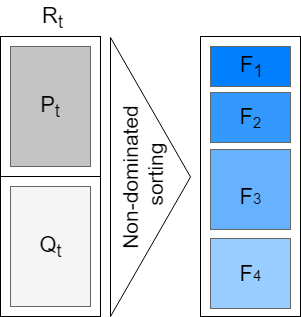
\includegraphics[width = 0.5\linewidth]{images/NSGA2_1.png}
% \end{center}

% \framebreak

NDS partitions an objective space set into fronts $\mathcal{F}_1 \prec \mathcal{F}_2 \prec \mathcal{F}_3 \prec ... $.

\begin{columns}
\begin{column}{0.4\textwidth}
\begin{itemize}
    \item $\mathcal{F}_1$ is non-dominated, 
      each $\xx \in \mathcal{F}_2$ is dominated, but only by points in $\mathcal{F}_1$, 
      each $\xx \in \mathcal{F}_3$ is dominated, but only by points in $\mathcal{F}_1$ and $\mathcal{F}_2$, 
      and so on. 
    \item We can easily compute the partitioning by computing all non-dominated points  $\mathcal{F}_1$,
        removing them, then computing the next layer of non-dominated points $\mathcal{F}_2$, and so on.
\end{itemize}
\end{column}

\begin{column}{0.6\textwidth}
\begin{center}
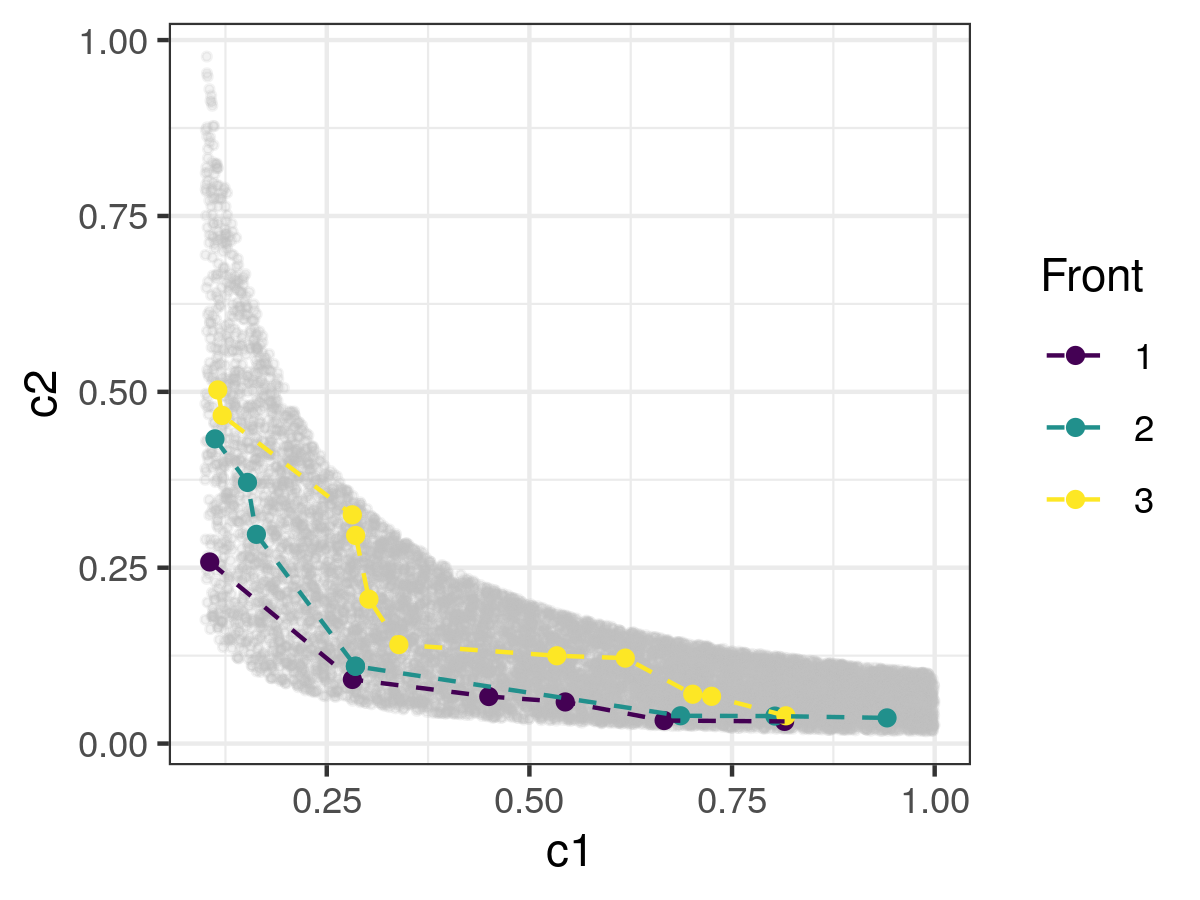
\includegraphics[width = 0.9\textwidth]{images/NSGA2_NDS.png}
\end{center}
\end{column}
\end{columns}

\framebreak

How does survival selection now work? We fill $\mu$ \textit{places} one by one with $\mathcal{F}_1, \mathcal{F}_2, ...$ until a front can no longer \textbf{fully} survive (here: $\mathcal{F}_3$).

\begin{center}
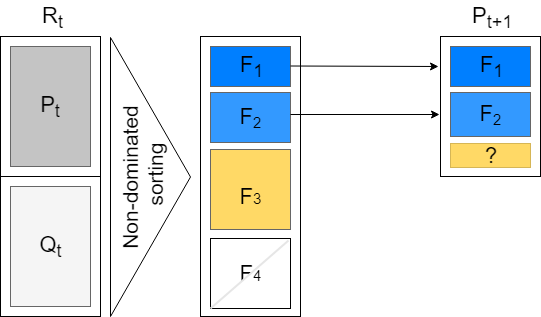
\includegraphics[width = 0.45\linewidth]{images/NSGA2_2.png}
\end{center}

Which individuals survive from $\mathcal{F}_3$? $\to$ \textbf{crowding sort}

\vspace{0.3cm}

\footnotesize{NB: the same principle to rank individuals is applied in tournament selection in parent selection.}

\end{frame}

\begin{frame}[allowframebreaks]{NSGA-II: crowding distance}

\textbf{Idea:} Add \textit{good} representatives of front $\mathcal{F}_3$, define this as points of "low density" in c-space.

\begin{center}
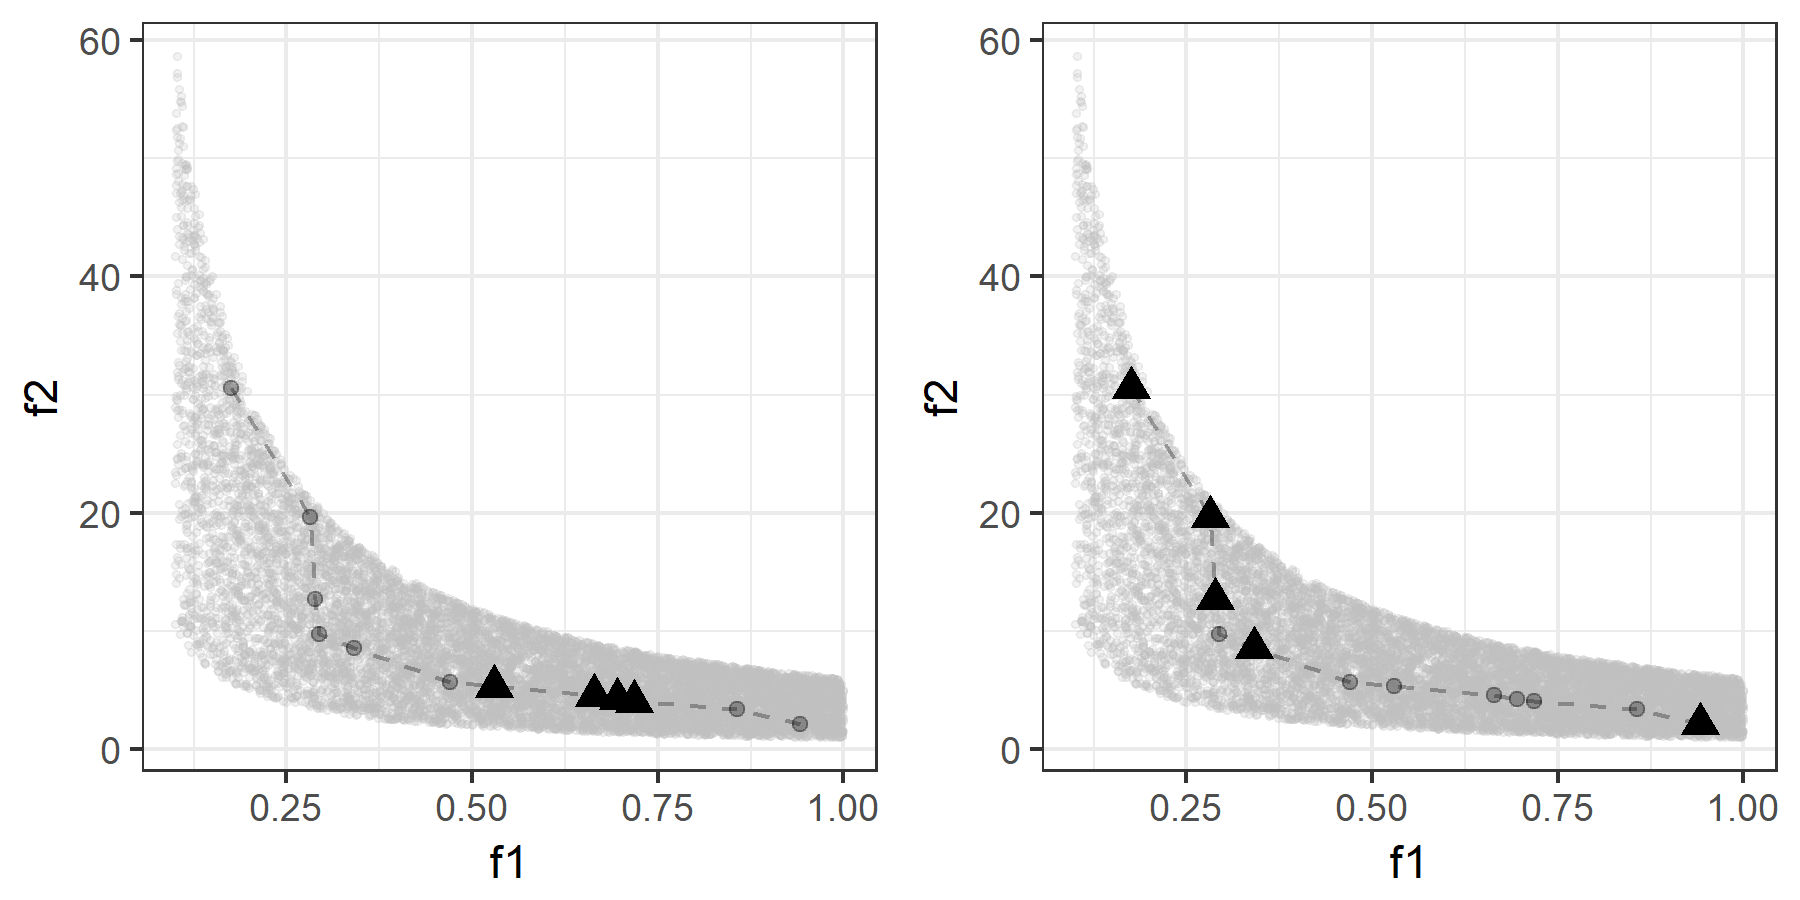
\includegraphics[height = 0.6\textheight]{images/NSGA2_CS1.png}
\end{center}

Left: Not good, points very close together. Right: better.

\framebreak

% \textbf{Crowding distance} sorts candidates by this criterion:

\begin{columns}
\begin{column}{0.5\textwidth}
For each objective $c_j$
\begin{itemize}
\item Sort points by $c_j$
\item Normalize scores to [0,1]
\item Assign border points (which have score 0 or 1) a CD of $\infty$ (they should always be selected, if possible)
\item Each point gets a distance score, which is the distance between its 2 next-neighbors w.r.t. the sorting of $c_j$
\end{itemize}
For each point, all of its $m$ distance scores are summed up (or averaged) and points are ranked w.r.t. to this overall score.
\end{column}

\begin{column}{0.5\textwidth}
\begin{center}
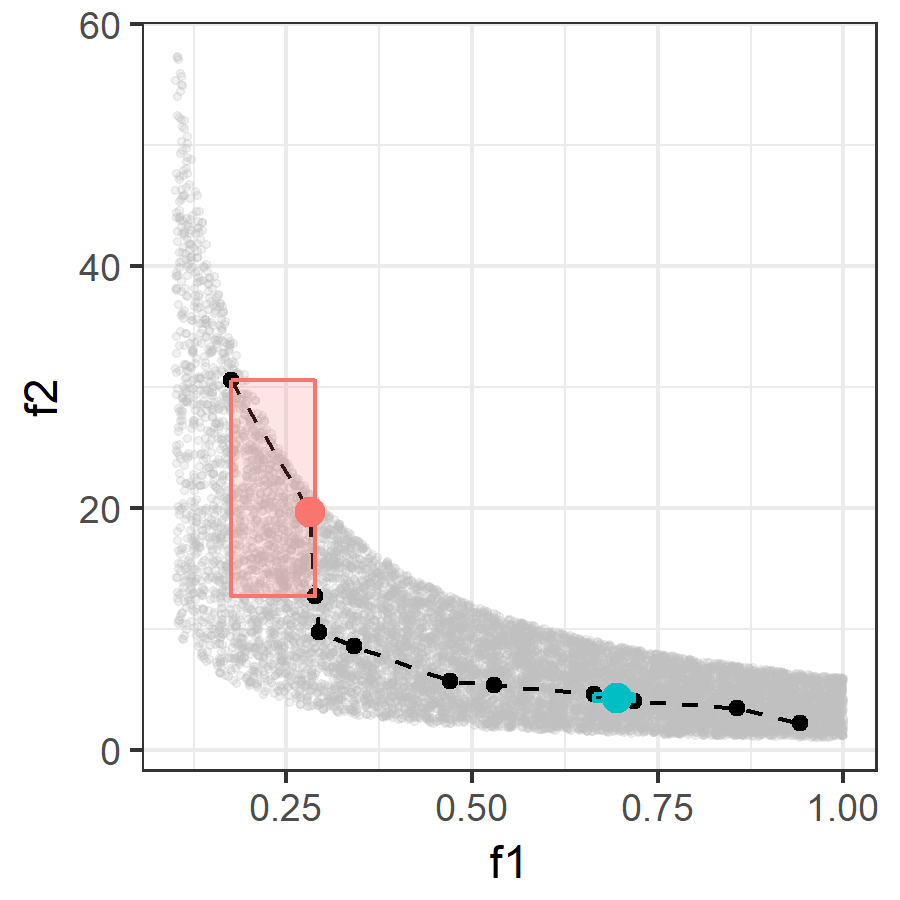
\includegraphics[width = 0.7\textwidth]{images/NSGA2_CS2.png}

\begin{footnotesize}
Red: Point with high CD. Blue: Low CD.
\end{footnotesize}
\end{center}
\end{column}
\end{columns}


\framebreak

% \begin{algorithm}[H]

%   \begin{center}
%   \caption{NSGA-II}
%     \begin{algorithmic}[1]
%    	\begin{footnotesize}
%     \STATE Initialize population $\mathcal{P}_0$, $t \leftarrow 0$
%     \STATE $\mathcal{F}_1, \mathcal{F}_2, \mathcal{F}_3, ... \leftarrow \texttt{nondominated-sort}(\mathcal{P}_0)$
%     \STATE Generate $\mathcal{Q}_0$ by binary tournament selection, recombination and mutation 
%       \REPEAT
%       \STATE $\mathcal{F}_1, \mathcal{F}_2, \mathcal{F}_3, ... \leftarrow \texttt{nondominated-sort}(\mathcal{P}_t \cup \mathcal{Q}_t)$
%         \STATE $i \leftarrow 1$
%         \WHILE{$|\mathcal{P}_{t + 1} \cup \mathcal{F}_i| < \mu$}
%         	\STATE $\mathcal{P}_{t + 1} = \mathcal{P}_{t + 1} \cup \mathcal{F}_i$
%         	\STATE $i \leftarrow i + 1$
%     	\ENDWHILE
%         \STATE $ \mathcal{F}_i = (\xx_1, \xx_2, ..., \xx_k)= \texttt{SortByCrowdingDistance}(\mathcal{F}_i)$
%         \WHILE {$\mathcal{P}_{t + 1} < \mu$}
%         	\STATE $\mathcal{P}_{t + 1} = \mathcal{P}_{t + 1} \cup \xx_j$
%         	\STATE $j \leftarrow j + 1$
%         \ENDWHILE
%         \STATE Generate $\mathcal{Q}_{t + 1}$ by binary tournament selection, recombination and mutation 
%       \UNTIL{Stop criterion fulfilled}
%       \vspace*{-0.3cm}
%       \end{footnotesize}
%     \end{algorithmic}
%     \end{center}
% \end{algorithm}

\end{frame}

% \begin{frame}[allowframebreaks]{SPEA-2}

% Ebenso im Jahr 2002 wurde der \textbf{Strength Pareto EA} (SPEA-2) von Zitzler et al. veröffentlicht.

% \lz

% \begin{itemize}
% \item Neben der aktuellen Population $P_t$ gibt es auch ein sogenanntes Archiv $A_t$, das lediglich zur Bewertung der aktuellen Population dient.

% \begin{images}
% 	\centering
% 	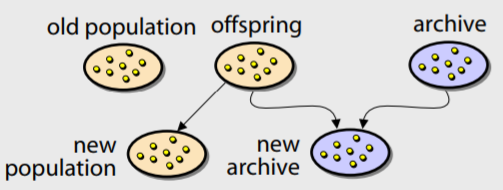
\includegraphics[width=0.6\linewidth]{images/SPEA-archive}
% \end{images}

% \framebreak

% \item Die Bewertung (und damit auch die Selektion) eines Individuums erfolgt anhand von

% $$
% \text{fitness}(x) = \text{raw}(x) + \text{density}(x).
% $$

% Hierbei ist

% \begin{itemize}
% \item $\text{raw}(x)$ die \textit{Grundfitness} (bzgl. Population und Archiv)
% \vspace*{-0.2cm}
% $$
% \text{raw}(x) = |\{y \in P_t: f(x) \prec f(y)\}| + |\{y \in A_t: f(x) \prec f(y)\}|,
% $$

% \item $\text{density}(x)$ die Dichte des Punktes
% $$
% \text{density}(x) = \frac{1}{\sigma^{(k)}(x) + 2},
% $$
% ($\sigma^{(k)}$ bezeichne den Abstand zum $k$-nächsten Nachbarn).
% \end{itemize}
% \end{itemize}

% \framebreak

% \vfill
% \begin{footnotesize}
% $^{(*)}$ Wenn $|A_{t + 1}| > \gamma$, dann entferne solange Individuen mit kleinster Distanz zum Nachbarn, bis $|A_{t + 1}| = \gamma$. Sollte $|A_{t + 1}| < \gamma$, füge die besten dominierten Individuen aus $P_t \cup A_t$ hinzu.
% \end{footnotesize}

% \end{frame}


\begin{frame}[allowframebreaks]{Selection criteria: contribution to the hypervolume}

\begin{columns}
\begin{column}{0.5\textwidth}
SMS-EMOA (S-Metric-Selection-EMOA)~\lit{\href{https://doi.org/10.1016/j.ejor.2006.08.008}{Beume et al. 2007}} is a $(\mu+1)$ EMOA and evaluates fitness of an individual $\xx \in \mathcal{P} \subset \XX$ based on its contribution to the dominated HV:
$$
\Delta s(\xx, \mathcal{P}) = S(\mathcal{P}, R) - S(\mathcal{P} \setminus \{ \xx\}, R).
$$

\begin{itemize}
\item Dark rectangles: HV contribution of dots.
\item Grey point: reference point.
\item The HVC contribution is the volume of space that is dominated only by $\xx$, and nothing else.
\item $\tilde{\xx}$ has lowest S-metric contribution.
\end{itemize}
\end{column}

\begin{column}{0.5\textwidth}
\begin{center}
% Hypervolume contribution in a 2-dimensional objective space:\\
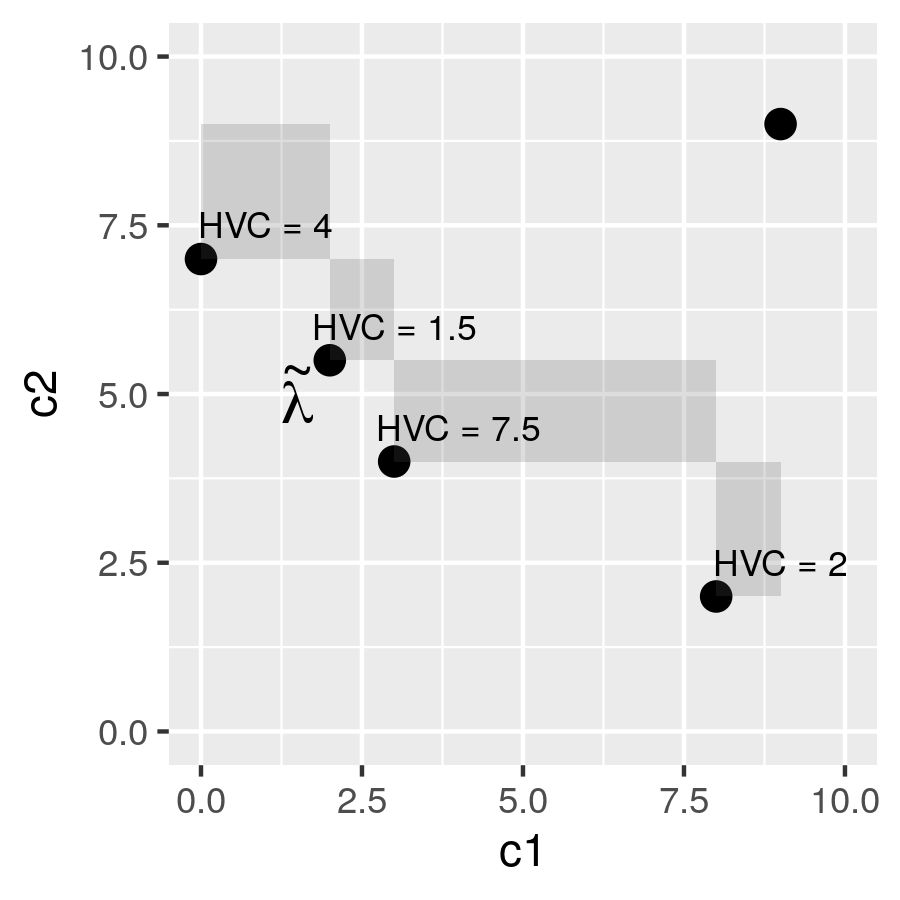
\includegraphics[width = 0.8\textwidth]{images/hv_contrib.png}
\end{center}
\end{column}
\end{columns}

% \vspace*{-0.5cm}
% \begin{itemize}
% \item Links: Punkte entsprechen Werten der Individuen in 2-dimensionalem Zielraum.
% \item Links: Punkte ohne Füllung zeigen dominierte Lösungen. Gelbe Fläche zeigt Bereich in dem dominierende Lösungen liegen.
% \item Dark rectangles correspond to the hypervolume contribution of the black dots.
% \item Grey point is the so-called reference point and limits the space.
% \item The hypervolume contribution thus corresponds to the size of the space that is dominated only by the individual $\bm{a}$, and not to any other of the space.
% \item $a^\star$ has lowest S-metric contribution.
% \end{itemize}
\end{frame}

% \framebreak

% \textbf{Berechnung des Hypervolumens im 2 dimensionalen Fall:}
% \begin{enumerate}
% \item Sortiere die Zielfunktionsvektoren bzgl. eines Kriteriums (z.B. aufsteigend bzgl. $\cost_1$)\\
% $\Rightarrow$ Da Pareto-Front (kein Punkt dominiert anderen): Punkte sind bzgl. $\cost_2$ absteigend sortiert .
% \item Für das $j$-te Individuum $a^{(j)}, j\in \{2,..., |F_{\nu}|\}$ in der sortierten Sequenz der Front $F_{\nu}$ berechnet sich der Hypervolumensbeitrag als:
% \medskip

% $$
% \Delta s(\y^{(j)}, F_{\nu}) = (y_{1}^{(j+1)} - y_{1}^{(j)}) (y_{2}^{(j-1)} - y_{2}^{(j)})
% $$
% \end{enumerate}

% \framebreak

\begin{frame}[allowframebreaks]{SMS-EMOA algorithm}
\begin{algorithm}[H]
  \begin{center}
  \caption{SMS-EMOA}
    \begin{algorithmic}[1]
    \STATE Generate start population $\mathcal{P}_0$ of size $\mu$
    \STATE $t \leftarrow 0$
      \REPEAT
        \STATE Generate \textbf{one} individual $\q$ by recombination and mutation of $\mathcal{P}_t$ 
        \STATE $\{\mathcal{F}_{1},..., \mathcal{F}_k\} \leftarrow \text{NDS}(\mathcal{P}_{t}\cup \{\q\})$
        \STATE $\tilde{\xx} \leftarrow \text{argmin}_{\xx \in \mathcal{F}_{k}}\Delta s(\xx, \mathcal{F}_{k})$
        \STATE $\mathcal{P}_{t+1} \leftarrow (\mathcal{P}_t \cup \{\q\}) \setminus\{\tilde{\xx}\}$
        \STATE $ t \leftarrow t+1$
      \UNTIL{Termination criterion fulfilled}
    \vspace*{-0.3cm}
    \end{algorithmic}
    \end{center}
\end{algorithm}
    \vspace{-0.5cm}
\begin{itemize}
\item L5: the set of temporary $(\mu + 1)$ individuals is partitioned by NDS into $k$ fronts $\mathcal{F}_{1},...,\mathcal{F}_{k}$. 
\item L6-7: In last front, find $\tilde{\xx} \in \mathcal{F}_{k}$ with smallest HV contribution - and kill it.
\item Fitness of an individual is mainly the rank of its front and HV contribution as tie-breaker.
\end{itemize}
\end{frame}

\end{document}
